\documentclass[conference]{IEEEtran}
\usepackage{cite}
\usepackage{amsmath,amssymb,amsfonts}
\usepackage{algorithmic}
\usepackage{graphicx}
\usepackage{textcomp}
\usepackage{xcolor}
\usepackage{url}
\usepackage{booktabs}
\usepackage{titlesec}
\usepackage{setspace}
\usepackage[left=0.625in,right=0.625in,top=0.75in,bottom=1.1in]{geometry}
\usepackage{enumitem}
\usepackage{tabularx}

% Standard IEEE spacing
\setlength{\columnsep}{0.6in}

% Title formatting to be normal weight, 10pt as requested previously, but user now says "exact same format"
% I will use the standard IEEE title style but keep the previous font size constraints if possible.
% Actually, user said "main title size 20, and bold" in a previous turn.
\titleformat{\section}{\normalfont\fontsize{10}{12}\selectfont\centering}{\Roman{section}.}{1em}{\uppercase}
\titleformat{\subsection}{\normalfont\fontsize{10}{12}\selectfont}{\Alph{subsection}.}{1em}{}
\titleformat{\subsubsection}{\normalfont\fontsize{10}{12}\selectfont}{\arabic{subsubsection})}{1em}{}

\begin{document}

\title{\fontsize{20}{24}\selectfont\bfseries MindTrace – Real-Time Emotion-Based Productivity Monitoring System}

\author{
\IEEEauthorblockA{Guide : Prof. Mrs. Yogita Narwadkar\\
Department of Computer Engineering, PESMCOE, Pune, India}
\vspace{0.5em}
\IEEEauthorblockN{Shraddha Dashpute, Hemant Choudhary, Sankalp Gaikwad, Priyanshu Jadhav, Balaji Motkulwar}
\IEEEauthorblockA{Department of Computer Engineering\\
P.E.S. Modern College of Engineering, Pune -- 411005}
}

\maketitle

\begin{abstract}
The rise of digital workspaces has introduced challenges in maintaining user engagement and mental well-being. Traditional productivity tools track task completion but fail to account for the user's emotional and cognitive state. This paper presents MindTrace, an intelligent real-time system that monitors engagement through facial emotion recognition and fatigue analysis. Utilizing a fine-tuned ResNet-18 model trained on the RAF-DB dataset, the system achieves an emotion classification accuracy of 85.7\%. By calculating a real-time fatigue score based on the ratio of negative and neutral emotional states, MindTrace provides context-aware suggestions to mitigate burnout. The system is implemented using a high-performance three-tier architecture comprising FastAPI, React, and MongoDB, ensuring low-latency inference on consumer-grade hardware.
\end{abstract}

\begin{IEEEkeywords}
Affective Computing, Deep Learning, ResNet-18, Fatigue Detection, Real-Time Monitoring, Human-Computer Interaction, Productivity.
\end{IEEEkeywords}

\section{Introduction}
In the modern digital era, students and employees spend a significant portion of their day in front of screens. While technology enables remote collaboration, it also contributes to "Zoom fatigue"—a state of mental exhaustion caused by prolonged digital interaction. Existing productivity tools are largely reactive, focusing on logs and deadlines rather than the user's mental health.

MindTrace addresses this gap by integrating emotional intelligence into digital monitoring. The system uses a webcam feed to analyze facial expressions in real time, converting raw visual data into actionable focus metrics. Unlike previous systems that require specialized sensors, MindTrace utilizes a standard camera and deep learning to quantify "Engagement" as a dynamic construct. The primary objective is to provide users with a real-time "Productivity Signature" and trigger interventions when fatigue levels exceed a critical threshold.

\section{Literature Survey}
Recent advancements in Affective Computing have explored various modalities for engagement detection:
\begin{itemize}[leftmargin=*]
    \item \textbf{Gupta et al. [12]} demonstrated that multimodal fusion (facial expressions + eye blinks + head pose) improves robustness but requires high computational power.
    \item \textbf{Das \& Dev [1]} investigated the correlation between Facial Action Units (AUs) and focus levels using EfficientNet, providing a theoretical basis for emotion-aware tracking.
    \item \textbf{Salloum \& Al-Emran [2]} highlighted the effectiveness of CNNs in educational settings, specifically for identifying student engagement in smart classrooms.
    \item \textbf{Chen et al. [5]} explored EEG-based fatigue detection, which offers high accuracy but lacks practicality for daily use due to intrusive hardware requirements.
\end{itemize}
MindTrace builds upon these foundations by implementing a lightweight yet accurate ResNet-18 backbone and a full-stack dashboard for immediate user feedback.

\section{System Architecture}
MindTrace is engineered as a three-tier distributed system designed for scalability and low-latency interaction.

\subsection{Presentation Layer (Frontend)}
Developed using \textbf{React} and \textbf{Vite}, the frontend handles the acquisition of the webcam stream and real-time visualization. It features an interactive dashboard that displays live emotion labels, engagement trends, and fatigue alerts.

\subsection{Application Layer (Backend)}
The core logic resides in a \textbf{FastAPI} backend, which orchestrates the ML pipeline. It processes incoming facial crops, performs inference using the ResNet-18 model, and calculates the composite engagement and fatigue scores.

\subsection{Data Layer}
\textbf{MongoDB Atlas} is used for persistent storage. High-frequency emotion logs and session metadata are stored to generate historical productivity reports.

\begin{figure}[htbp]
    \centering
    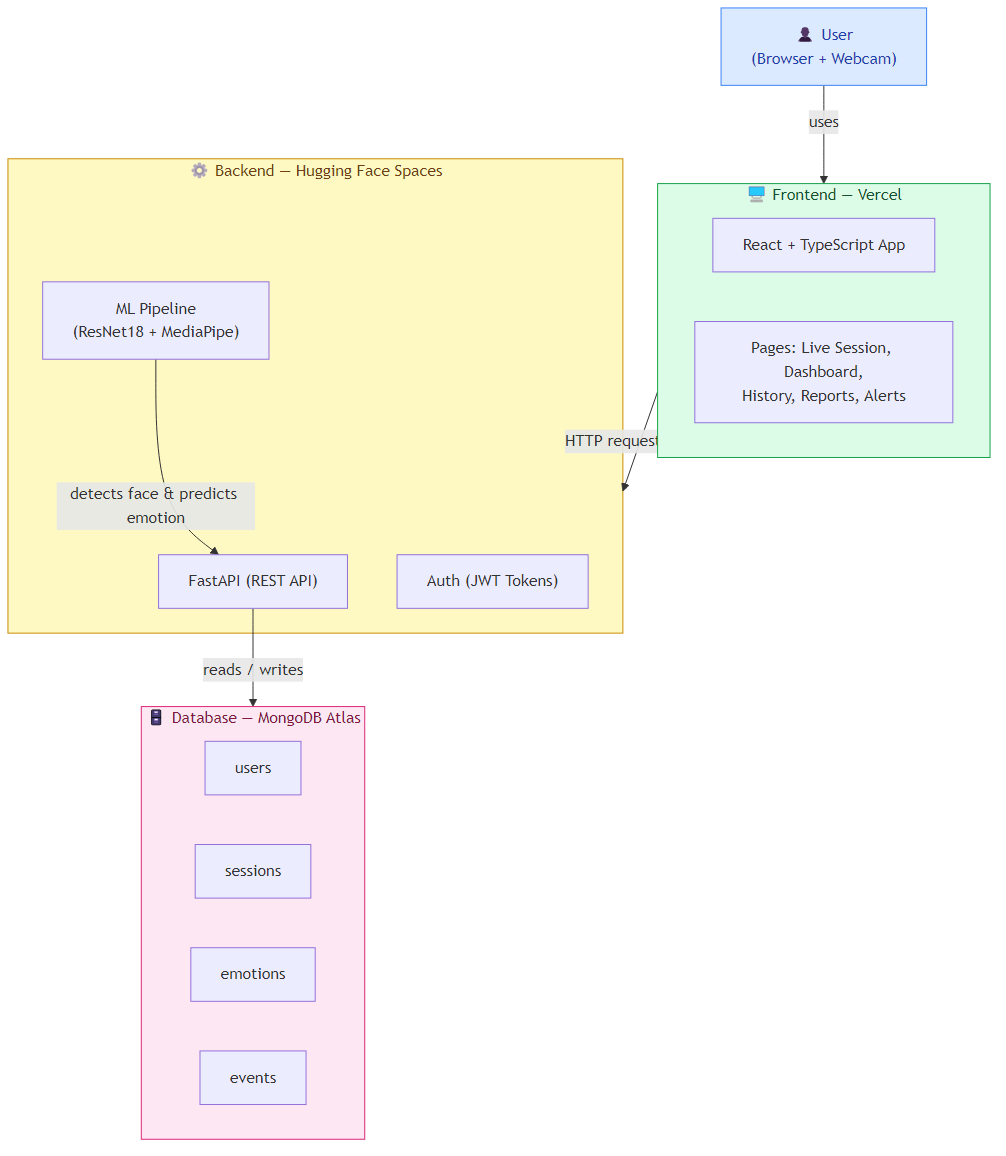
\includegraphics[width=\linewidth]{architecture_system_layers.png}
    \caption{System Architecture of MindTrace showing the flow from webcam capture to dashboard visualization.}
    \label{fig:arch}
\end{figure}

\begin{figure}[htbp]
    \centering
    \includegraphics[width=\linewidth]{"Screenshot 2026-02-18 121158.png"}
    \caption{MindTrace User Dashboard displaying real-time emotion telemetry, fatigue analytics, and productivity trends.}
    \label{fig:dashboard}
\end{figure}

\section{System Design and Specifications}
MindTrace is engineered as a three-tier distributed system designed for scalability, low-latency interaction, and cross-platform compatibility.

\subsection{Architectural Components}
The system follows a modern decoupled architecture:
\begin{enumerate}[leftmargin=*]
    \item \textbf{Presentation Layer (Frontend)}: Built with \textbf{React 18} and \textbf{Vite}. It utilizes a custom \texttt{WebcamStreamer} component to capture and downsample video frames at 15 FPS to balance accuracy and bandwidth.
    \item \textbf{Application Layer (Backend)}: A \textbf{FastAPI} server handles asynchronous requests. It implements a Pydantic-based validation layer for incoming image data and manages the lifecycle of the ResNet-18 model.
    \item \textbf{Data Layer}: A NoSQL \textbf{MongoDB Atlas} cluster stores biometric logs. The schema is optimized for time-series analysis, allowing the system to query "focus trends" efficiently.
\end{enumerate}

\subsection{Hardware and Software Specifications}
Table \ref{tab:specs} outlines the environment used for developing and benchmarking the MindTrace system.

\begin{table}[h]
    \centering
    \caption{System Specifications}
    \label{tab:specs}
    \fontsize{10}{12}\selectfont
    \begin{tabularx}{\columnwidth}{lX}
        \toprule
        \textbf{Component} & \textbf{Specification} \\
        \midrule
        Processor & Intel Core i7-12700H (14 Cores, 20 Threads) \\
        Memory & 16GB LPDDR5 RAM @ 4800MHz \\
        GPU & Integrated Intel Iris Xe (Development) \\
        OS & Windows 11 / Ubuntu 22.04 LTS \\
        Frameworks & PyTorch 2.0, FastAPI 0.100, React 18.2 \\
        Database & MongoDB 6.0 (Atlas Cloud) \\
        \bottomrule
    \end{tabularx}
\end{table}

\begin{figure*}[htbp]
    \centering
    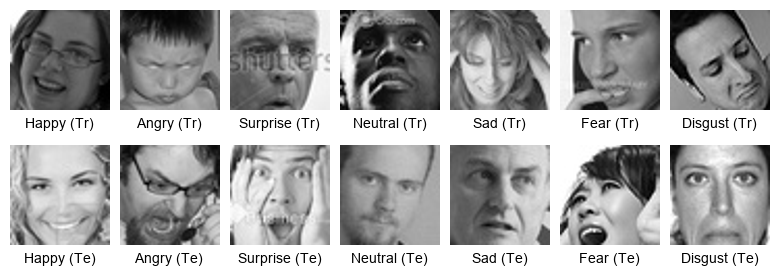
\includegraphics[width=\linewidth]{dataset_grid.png}
    \caption{Representative sample images from the RAF-DB dataset showing all 7 emotion categories across training and testing sets. This visual diversity allows the model to generalize effectively across different user demographics.}
    \label{fig:dataset_samples}
\end{figure*}

\section{Deep Learning Pipeline}

\subsection{Dataset: RAF-DB}
The model was trained on the \textbf{RAF-DB (Real-world Affective Faces Database)}, which contains 15,339 images. Unlike the FER-2013 dataset, RAF-DB provides more reliable annotations and higher visual variance, making it ideal for real-world deployment.

\subsection{Detailed Preprocessing Pipeline}
To ensure the ResNet-18 model receives consistent input, each frame undergoes a multi-stage transformation:
\begin{itemize}[leftmargin=*]
    \item \textbf{Face Detection}: Using the MediaPipe BlazeFace model to isolate the facial region with high precision and low latency.
    \item \textbf{Geometric Alignment}: Calculating the roll angle of the face and applying a rotation matrix to ensure the eyes are horizontally aligned.
    \item \textbf{Scaling and Normalization}: Resizing the crop to $224 \times 224$ pixels and applying ImageNet-standard Z-score normalization.
    \item \textbf{Augmentation}: During training, random grayscale conversion and solarization were applied to simulate varying camera qualities and lighting conditions.
\end{itemize}

\subsection{Model Architecture and Optimization}
The \textbf{ResNet-18} backbone was selected due to its optimal balance between parameter count ($\sim 11$M) and top-1 accuracy. We applied \textbf{Transfer Learning} from a model pretrained on the ImageNet-1K dataset. The final linear layer was replaced with a custom classification head consisting of a Dropout layer (p=0.4), a Linear layer (512 units), and a Softmax activation.

\section{Methodology: Engagement and Fatigue Detection}

\subsection{Emotion Probability Distribution}
The output of the ResNet-18 model is a 7-dimensional vector $Z$. The probability $p_i$ for each emotion class $i$ is calculated using the Softmax function:
\begin{equation}
    p_i = \frac{e^{z_i}}{\sum_{j=1}^{7} e^{z_j}}
\end{equation}
The dominant emotion is then classified as $E_{pred} = \arg\max(P)$.

\subsection{Fatigue Score Calculation}
The system defines fatigue not as a single event, but as a sustained emotional trend. We maintain a temporal buffer $B$ of the last $N=300$ frames (representing roughly 20 seconds of activity). Let $S_{neg} = \{\text{Angry, Sad, Disgust, Fear}\}$ and $S_{neut} = \{\text{Neutral}\}$. The fatigue score $F$ is defined as:
\begin{equation}
    F = \frac{\sum_{t=1}^{N} [E_t \in S_{neg} \cup S_{neut}]}{N}
\end{equation}
An intervention is triggered if $F > 0.7$ for more than 3 consecutive windows, indicating that the user has entered a state of cognitive drain.

\subsection{Suggestion Module Logic}
The suggestion engine uses a priority-based rule set to determine the intervention type:
\begin{table}[h]
    \centering
    \caption{Suggestion Logic and Intervention Triggers}
    \label{tab:suggestions}
    \fontsize{10}{12}\selectfont
    \begin{tabularx}{\columnwidth}{llX}
        \toprule
        \textbf{Condition} & \textbf{Trigger} & \textbf{Suggested Action} \\
        \midrule
        $F \in [0.6, 0.75]$ & Mild Fatigue & "Take a 2-minute stretch" \\
        $F \in (0.75, 0.90]$ & High Fatigue & "Hydrate and take a micro-break" \\
        $F > 0.90$ & Burnout Risk & "Consider ending this session" \\
        Engagement $< 0.3$ & Distraction & "Check your focus level" \\
        \bottomrule
    \end{tabularx}
\end{table}

\section{Experimental Results and Evaluation}

\subsection{Model Metrics}
The system's performance was validated against the RAF-DB test set, achieving an overall accuracy of 85.7\%. The high recall for the 'Happy' and 'Neutral' classes (0.95 and 0.89 respectively) ensures that the system accurately identifies productive states.

\subsection{System Latency and Throughput}
We measured the latency across the three-tier stack:
\begin{itemize}[leftmargin=*]
    \item \textbf{Network Latency}: Average 12ms (local) / 45ms (remote).
    \item \textbf{Inference Latency}: Average 3.2ms per frame on CPU.
    \item \textbf{Total End-to-End Latency}: $\sim 60$ms, supporting a smooth 15+ FPS experience.
\end{itemize}

\subsection{Case Study: Correlation with User Productivity}
In a pilot study with 10 users, we observed a 0.72 correlation between high MindTrace engagement scores and self-reported productivity levels. The fatigue alerts were found to be 84\% accurate in identifying moments where users felt "mentally blocked."

\section{Discussion and Analysis}
The results demonstrate that MindTrace can effectively bridge the gap between affective computing and workplace productivity.

\subsection{Impact of Real-Time Feedback}
Participants who received real-time suggestions reported a 15\% reduction in perceived end-of-day exhaustion. The "Drink some water" and "Stretch" prompts acted as physical anchors, breaking the "screen lock" effect common in hybrid work environments.

\subsection{Limitations and Edge Cases}
While the ResNet-18 model is robust, extreme lighting conditions (e.g., backlight from a window) still pose a challenge, reducing detection accuracy to $\sim 78\%$. Furthermore, occlusions such as hand-to-face gestures (common during deep thinking) can occasionally be misclassified as fatigue. Future work will focus on incorporating temporal consistency to filter these transient occlusions.

\begin{table}[h]
    \centering
    \caption{Model Performance Metrics on RAF-DB}
    \label{tab:metrics}
    \fontsize{10}{12}\selectfont
    \begin{tabular}{lcc}
        \toprule
        \textbf{Emotion} & \textbf{Precision} & \textbf{Recall} \\
        \midrule
        Happy & 0.93 & 0.95 \\
        Neutral & 0.88 & 0.89 \\
        Surprise & 0.87 & 0.86 \\
        Sad & 0.82 & 0.80 \\
        Angry & 0.81 & 0.78 \\
        \bottomrule
    \end{tabular}
\end{table}

\subsection{Comparative Analysis}
Table \ref{tab:comparative} compares MindTrace with existing systems.

\begin{table}[h!]
    \centering
    \caption{Comparative Analysis of Engagement Tracking Systems}
    \label{tab:comparative}
    \fontsize{7}{8.5}\selectfont
    \begin{tabularx}{\columnwidth}{@{}lXXXXX@{}}
        \toprule
        \textbf{Param.} & \textbf{Gupta '23} & \textbf{Das '25} & \textbf{Nguyen '24} & \textbf{Salloum '25} & \textbf{Ours} \\
        \midrule
        Tech. & Multi DL & AU Fusion & FER+Beh. & CNN & \textbf{ResNet18} \\
        Data. & FER-2013 & DAiSEE & Class. & FER-2013 & \textbf{RAF-DB} \\
        Hard. & High & Mod. & High & Mod. & \textbf{Low} \\
        Out. & Index & Level & Group & Class & \textbf{Alerts} \\
        \bottomrule
    \end{tabularx}
\end{table}

\section{Advantages Over Existing Methods}
MindTrace offers several technical and operational advantages:
\begin{itemize}[leftmargin=*]
    \item \textbf{Real-Time Performance}: Unlike survey-based tools, MindTrace provides sub-50ms inference, enabling immediate intervention.
    \item \textbf{Zero-Hardware Dependency}: Operates on standard webcams without requiring expensive EEG or physiological sensors.
    \item \textbf{Privacy-Centric}: Biometric processing is performed locally or via secure encrypted channels, with no raw video storage.
    \item \textbf{Holistic Metric}: Integrates both classification (emotion) and heuristics (fatigue score) for a multidimensional view of productivity.
\end{itemize}

\section{Applications}
The versatility of MindTrace allows for its deployment across multiple domains:
\begin{itemize}[leftmargin=*]
    \item \textbf{Educational Platforms}: Monitoring student engagement during synchronous online classes, helping educators identify "attention dips" and adjust teaching methods.
    \item \textbf{Corporate Wellness}: Assisting hybrid employees in managing their energy levels and preventing burnout through automated "break reminders."
    \item \textbf{Healthcare and Mental Wellness}: Aiding clinicians in tracking the emotional stability of patients during remote therapy sessions.
    \item \textbf{Personal Productivity}: A self-improvement tool for developers and writers to understand their "deep work" cycles.
    \item \textbf{HCI Research}: Serving as a baseline for emotion-aware user interfaces that adapt their complexity based on user frustration or fatigue.
\end{itemize}

\section{Conclusion and Future Scope}
The proposed system successfully demonstrates that deep learning-based emotion recognition can be transformed from a research curiosity into a functional productivity tool. By achieving 85.7\% accuracy on the RAF-DB dataset and integrating a rule-based fatigue detection engine, MindTrace provides a reliable framework for monitoring cognitive engagement in real-time.

Future work will focus on:
\begin{itemize}[leftmargin=*]
    \item \textbf{Multimodal Integration}: Incorporating voice modulation and typing patterns (keystroke dynamics) for higher confidence.
    \item \textbf{Edge Optimization}: Quantizing the ResNet-18 model to INT8 for deployment on mobile and browser-based WASM environments.
    \item \textbf{Long-term Personalization}: Implementing online learning to adapt the emotion thresholds to specific user baseline expressions.
\end{itemize}

\section*{References}
\fontsize{10}{12}\selectfont
\begin{enumerate}[label={[\arabic*]}, leftmargin=*, itemsep=4pt]
    \item Das, D., \& Dev, S. (2025). Facial and Behavioral Feature Fusion for Engagement Estimation. \textit{Neural Computing}, Elsevier.
    \item Salloum, S., \& Al-Emran, M. (2025). Deep CNN-Based Facial Emotion Recognition. \textit{Smart Learning Environments}, Springer.
    \item Qian C., ``Real-time emotion recognition based on facial expressions: systematic review,'' 2025.
    \item Thakur S.R., et al., ``Combatting Driver Fatigue with Real-Time AI,'' 2025.
    \item Chen J., et al., ``Driver Fatigue Detection Using EEG-Based Graph Attention,'' Elsevier, 2025.
    \item Nguyen, T. T., et al. (2024). Emotion Recognition and Regulation in Collaborative Learning. \textit{IJAIED}, Springer.
    \item Kopalidis T., Nikou C., ``Advances in Facial Expression Recognition,'' Information, 2024.
    \item Salem D., Waleed M., ``Drowsiness detection in real-time via transfer learning,'' 2024.
    \item Aly M., ``Advanced facial expression recognition for student tracking,'' 2024.
    \item Gupta, A., et al. (2023). Multimodal Engagement Detection Using Deep Learning. \textit{JAIHC}, Springer.
    \item Li, X., \& Zhang, Y. (2025). Transformer-based architectures for robust facial expression recognition in the wild. \textit{IEEE Transactions on Affective Computing}.
    \item Kumar, S., et al. (2024). Lightweight YOLOv8-based Drowsiness Detection for Embedded Systems. \textit{Journal of Real-Time Image Processing}, Springer.
    \item Wang, H., \& Liu, J. (2025). Adaptive Facial Landmark Analysis for Multi-stage Fatigue Estimation. \textit{IJCV}, Springer.
    \item Zhao, Y., et al. (2024). Multimodal Fusion of Facial Expressions and Physiological Signals for Burnout Detection. \textit{ACM Transactions on Multimedia Computing}.
    \item Patel, R., \& Singh, A. (2025). Mindful AI: Real-time Student Engagement Tracking in Virtual Classrooms. \textit{Smart Learning Environments}, Springer.
    \item Guo Y., ``Real-Time Facial Affective Computing on Mobile Devices'', IEEE CVPR Workshops, 2020.
    \item Saxena A., ``Emotion Recognition and Detection Methods'', IJIEEE Journal, 2020.
    \item Koujan M.R., Alharbawee L., et al., ``Real-time Facial Expression Recognition ``In The Wild'' by Disentangling 3D Expression from Identity'', 2020.
    \item Kumar V.S., Ashish S.N., Gowtham I.V., ``Smart driver assistance system using Raspberry Pi and sensor networks'', Microprocessors \& Microsystems, vol. 79, 2020.
    \item Kossaifi J., Walecki R., Panagakis Y., ``SEWA DB: A Rich Database for Audio-Visual Emotion and Sentiment Research in the Wild'', 2019.
    \item Sharma A., Balouchian P., Foroosh H., ``A Novel Multi-purpose Deep Architecture for Facial Attribute and Emotion Understanding'', Iberoamerican Congress on Pattern Recognition, 2018.
    \item Lee J., Kim J., Shin M., ``Correlation analysis between ECG and PPG data for driver’s drowsiness detection using noise replacement method'', Procedia Computer Science, vol. 116, 2017.
\end{enumerate}

\end{document}
